
\begin{figure*}
\centering
\subfloat[Figure A][\label{fig:webrtcA}
$p_1$ connects to $p_2$ using the signaling service. 
1: $p_1$ pushes its offer ticket; 
2: $p_2$ pulls the ticket; 
3: $p_2$ pushes its response; 
4: $p_1$: pulls the response and establishes a 
bidirectional connection with $p_2$. $p_3$ does the same with $p_2$. Figure~\ref{fig:webrtcB} depicts the resulting network.]{
  
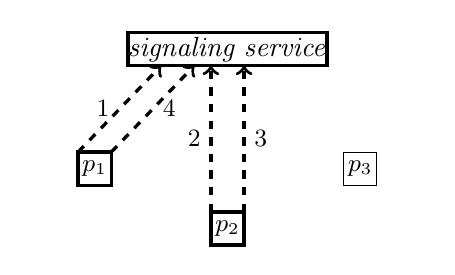
\begin{tikzpicture}[scale=1.2]

\newcommand\X{40pt};
\newcommand\Y{18pt};

\draw( 1.5*\X, 0); %% spacing
\draw(-1.5*\X, 0); %% spacing

\draw[fill=white,very thick](0*\X, 0*\Y) 
node{\emph{signaling service}} +(-30pt,-5pt) rectangle +(30pt,5pt);

\small
\draw[->,dashed, very thick](-5 -1*\X, 5-2*\Y) --
node[anchor=east]{1} (-20pt,-5pt);
\draw[->,dashed, very thick]( 5 -1*\X, 5-2*\Y) --
node[anchor=west]{4} (-10pt,-5pt);

\draw[->,dashed, very thick](-5pt,  5-3*\Y) --
node[anchor=east]{2}(-5pt,-5pt);
\draw[->,dashed, very thick](5pt , 5-3*\Y) --
node[anchor=west]{3} (5pt,-5pt);


\draw[fill=white, very thick]
(-1*\X,-2*\Y) node{$p_1$} +(-5pt,-5pt) rectangle +(5pt,5pt);
\draw[fill=white, very thick]
(0*\X, -3*\Y) node{$p_2$} +(-5pt,-5pt) rectangle +(5pt,5pt);
\draw[fill=white] (1*\X, -2*\Y) node{$p_3$} +(-5pt,-5pt) rectangle +(5pt,5pt);

\end{tikzpicture}

% \begin{tikzpicture}
% \matrix (m) [matrix of math nodes,row sep=4em,column sep=4em] {
% \node(ss)[draw]{signaling}; & \node(p3)[draw]{p3}; \\
% \node(p1)[draw]{p1}; & \node(p2)[draw]{p2}; \\
% };
% \path[->]
%   (p2) edge[dashed] node[fill=white]{1:emit} (ss)
%   (p3) edge[dashed] node[fill=white,bend left]{2:pull} (ss)
%   (p3) edge[dashed, bend right] node[fill=white]{3:accept} (ss)
%   (p2) edge[dashed,bend left] node[fill=white]{4:pull} (ss)
%   (p3) edge[<->,thick] node[fill=white,right]{5:connected} (p2);
% \end{tikzpicture}}
\hspace{5pt}
\subfloat[Figure B][\label{fig:webrtcB}
$p_1$ connects to $p_3$ using $p_2$ as mediator. 
1: $p_1$ sends its offer ticket to $p_2$; 
2: $p_2$ forwards it to $p_3$ and registers $p_1$ as the emitter; 
3: $p_3$ sends its response to $p_2$; 
4: $p_2$ forwards it to the emitter $p_1$ which connects to $p_3$.]{
  
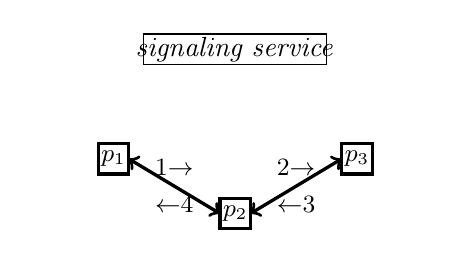
\begin{tikzpicture}[scale=1.1]

\newcommand\X{40pt};
\newcommand\Y{18pt};

\draw(1.7*\X, 0); %% spacing
\draw(-1.7*\X, 0); %% spacing

\draw[fill=white](0*\X, 0*\Y)
node{\emph{signaling service}} +(-30pt,-5pt) rectangle +(30pt,5pt);

\small
\draw[<->, very thick](5-1*\X,-2*\Y)--
node[anchor=south]{1$\rightarrow$}
node[anchor=north]{$\leftarrow$4}(-5pt,-3*\Y);
\draw[<->, very thick](5pt,-3*\Y)--
node[anchor=south]{2$\rightarrow$}
node[anchor=north]{$\leftarrow$3}(-5+1*\X,-2*\Y);

\draw[fill=white, very thick]
(-1*\X,-2*\Y) node{$p_1$} +(-5pt,-5pt) rectangle +(5pt,5pt);
\draw[fill=white, very thick]
(0*\X, -3*\Y) node{$p_2$} +(-5pt,-5pt) rectangle +(5pt,5pt);
\draw[fill=white, very thick]
(1*\X, -2*\Y) node{$p_3$} +(-5pt,-5pt) rectangle +(5pt,5pt);

\end{tikzpicture}

% \begin{tikzpicture}
% \matrix (m) [matrix of math nodes,row sep=4em,column sep=4em] {
% \node(ss)[draw]{signaling}; & \node(p3)[draw]{p3}; \\
% \node(p1)[draw]{p1}; & \node(p2)[draw]{p2}; \\
% };
% \path[->]
%   (p1) edge[dashed,bend left] node[fill=white]{1:emit} (p2)
%   (p2) edge[dashed,bend left] node[fill=white,left]{2:emit/p1} (p3)
%   (p3) edge[dashed,bend left] node[fill=white,right]{3:accept/p1} (p2)
%   (p2) edge[dashed,bend left] node[fill=white]{4:accept} (p1)
%   (p1) edge[<->,thick] (p2)
% %  (p1) edge[<->,thick,bend left] (p3)
%   (p2) edge[<->,thick]  (p3);

% \end{tikzpicture}}
\hspace{5pt}
\subfloat[Figure C][The resulting network overlay: a fully connected network
composed of 3 members.]{
  
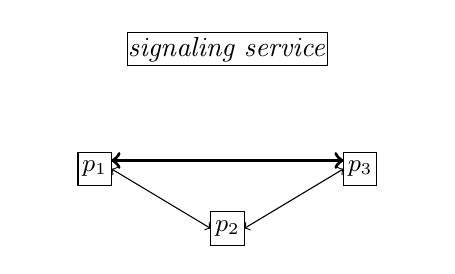
\begin{tikzpicture}[scale=1.2]

\newcommand\X{40pt};
\newcommand\Y{18pt};

\draw(1.5*\X, 0); %% spacing
\draw(-1.5*\X, 0); %% spacing

\draw[fill=white](0*\X, 0*\Y)
node{\emph{signaling service}} +(-30pt,-5pt) rectangle +(30pt,5pt);

\small
\draw[<->](5-1*\X,-2*\Y)--(-5pt,-3*\Y);
\draw[<->](5pt,-3*\Y)--(-5+1*\X,-2*\Y);
\draw[<->, very thick](5 - 1*\X, 2.5 -2*\Y)--(-5+1*\X, 2.5 -2*\Y);

\draw[fill=white]
(-1*\X,-2*\Y) node{$p_1$} +(-5pt,-5pt) rectangle +(5pt,5pt);
\draw[fill=white]
(0*\X, -3*\Y) node{$p_2$} +(-5pt,-5pt) rectangle +(5pt,5pt);
\draw[fill=white]
(1*\X, -2*\Y) node{$p_3$} +(-5pt,-5pt) rectangle +(5pt,5pt);

\end{tikzpicture}


% \begin{tikzpicture}
% \matrix (m) [matrix of math nodes,row sep=4em,column sep=4em] {
% \node(ss)[draw]{signaling}; & \node(p3)[draw]{p3}; \\
% \node(p1)[draw]{p1}; & \node(p2)[draw]{p2}; \\
% };
% \path[->]
%   (p1) edge[<->,thick] (p2)
%   (p1) edge[<->,thick] (p3)
%   (p2) edge[<->,thick]  (p3);
% \end{tikzpicture}}
\caption{\label{fig:webrtc}Creating an overlay network on top of WebRTC.}
\end{figure*}


\section{Related work}
\label{sec:relatedwork}


WebRTC allows real-time peer-to-peer communication between browsers even when 
complex network systems such as firewalls, proxies or Net Address Translation
(NAT) are involved. However, WebRTC does not manage addressing nor routing. To
establish a connection, the browsers exchange offers and acknowledgments
through a common mediator, e.g., mails, dedicated signaling services
\footnote{\url{http://peerjs.com/}},
existing WebRTC connections\footnote{\url{http://ozan.io/p/}} etc. In
figure~\ref{fig:webrtc}, $p_2$ wants to connect to $p_3$. Therefore, $p_2$
pushes an offer ticket to a signaling service\footnote{Many signaling services
  can exist}. Peer $p_3$ pulls the offers, stamps it and pushes it back to the
signaling service. Finally, $p_2$ pulls the stamped ticket and establishes a
bidirectional connection with $p_3$.  Identically, $p_1$ establishes a
connection to $p_2$. This round-trip procedure is called \emph{three-way
  handshake}. At this point, Peer $p_1$ is able to establish a connection to
$p_3$ without the mediation of the signaling service. Peer $p_1$ pushes an
offer ticket to $p_2$.  As $p_2$ is already connected to $p_1$, it forwards the
offer to $p_3$ and registers $p_1$ as the emitter. Peer $p_3$ stamps the ticket
and sends it back to $p_2$ who then forwards it to $p_1$. Upon receipt, $p_1$
establishes a bidirectional connection with $p_3$. Notice that if $p_2$
crashes during the forwarding process, the connection establishment will fail,
even if an alternative route exists as WebRTC does not manage routing.

Using signaling services and existing WebRTC connections allows deploying
random peer sampling protocols~\cite{jelasity2004peer} easily on browsers that
can run on mobile phones or tablets connected to mobile networks. In this
context, it is crucial to keep the number of connections as low as possible in
order to reduce traffic usage and limit resource consumption.

Random peer sampling protocols~\cite{jelasity2004peer} provide each
peer with a partial view $\mathcal{P}$ of the network membership
$\mathcal{N}$. They populate the partial views with references to
peers chosen at random among $\mathcal{N}$ following a uniform
distribution using local knowledge only. Their goal is to converge to
an overlay network exposing properties similar to random
graphs~\cite{erdos1959random}. They efficiently provide connectedness,
robustness, messages dissemination etc. A wide variety of gossip-based
protocols use random peer sampling (e.g. topology
management~\cite{voulgaris2005epidemic, jelasity2009tman,
  dabek2004vivaldi}).

Representatives of random peer sampling
protocols~\cite{voulgaris2005cyclon, eugster2003lightweight,
  tolgyeski2009adaptive} use a fixed-size partial view. Therefore, they
have to know \emph{a priori} the maximum order of magnitude of the
network size to set their appropriate parameters. These decisions
cannot be safely retracted afterwards. For this reason, the partial
views are commonly oversized compared to the actual network
size. Consequently, it is possible for a browser to maintain 10
connections with others while only 6 are required. In WebRTC context,
we need a dynamic peer sampling service able to adapt to the number of
participants.

Network size estimators can be used to introduce adaptiveness in peer
sampling. These approaches either use
\begin{inparaenum}[(i)]
\item sampling techniques~\cite{mane05network, ganesh2007peer,
    kostoulas2007active} which analyze a network subset and deduce the network
  size using probabilistic functions,
\item sketching techniques~\cite{flajolet2008hyperloglog, baquero2012extrema}
  which use hashing to compress the high amount of data and deduce the network
  size using the collisions,
\item averaging techniques~\cite{jelasity2004epidemic, blasa2011symmetric}
  which use aggregations that converge over exchanges to a value which depends
  of the network size.
\end{inparaenum}
Unfortunately, while they can be very precise in their estimate, they
imply a communication overhead and may have strong assumptions
(e.g. random graph topology). In WebRTC context, adaptiveness should
introduce a minimum overhead in peer sampling.

%% figure related to proposal, here to be on top of page
\begin{figure*}
  \centering
  \subfloat[Figure A][$p_1$ contacts $p_2$ to join the network. $p_1$ adds
  $p_2$ to its neighborhood. $p_1$ sends its request to $p_2$.]{
    
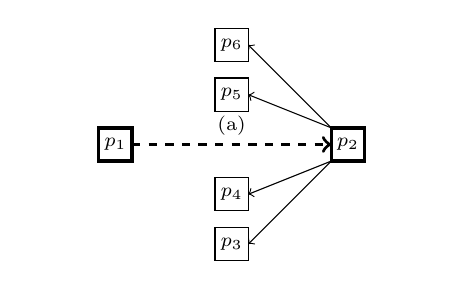
\begin{tikzpicture}[scale=1.2]

  \newcommand\X{35pt};
  \newcommand\Y{15pt};

  \draw(-0.75*\X, 0pt); %% positioning
  \draw( 2.75*\X, 0pt); %% positioning

  \scriptsize
  \draw[->,dashed,very thick](5+0*\X, 0*\Y) -- 
  node[anchor=south]{(a)}(-5+ 2*\X, 0*\Y);
  \draw[->] (-5+2*\X, 5pt) -- (5+\X, \Y);
  \draw[->] (-5+2*\X, 5pt) --  (5+\X, 2*\Y);
  \draw[->] (-5+2*\X, -5pt) -- (5+\X, -\Y);
  \draw[->] (-5+2*\X, -5pt) -- (5+\X, -2*\Y);

  \draw[fill=white, very thick]
  (0*\X, 0*\Y) node{$p_1$} +(-5pt,-5pt) rectangle +(5pt,5pt);
  \draw[fill=white, very thick]
  (2*\X, 0*\Y) node{$p_2$} +(-5pt,-5pt) rectangle +(5pt,5pt);

  \draw[fill=white](1*\X,2*\Y) node{$p_6$} +(-5pt,-5pt) rectangle +(5pt,5pt);
  \draw[fill=white](1*\X,1*\Y) node{$p_5$} +(-5pt,-5pt) rectangle +(5pt,5pt);
  \draw[fill=white](1*\X,-1*\Y) node{$p_4$} +(-5pt,-5pt) rectangle +(5pt,5pt);
  \draw[fill=white](1*\X,-2*\Y) node{$p_3$} +(-5pt,-5pt) rectangle +(5pt,5pt);
  
\end{tikzpicture}}
  \hspace{8pt}
  \subfloat[Figure B][The $onSubs(p_1)$ event is raised at $p_1$
  which forwards the subscription to $p_1$'s neighborhood.]{
    
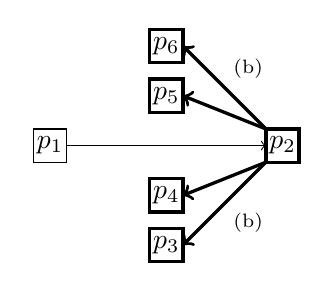
\begin{tikzpicture}[scale=1.2]

  \newcommand\X{35pt};
  \newcommand\Y{15pt};

  \scriptsize
  \draw[->](5+0*\X, 0*\Y) -- (-5+ 2*\X, 0*\Y);
  \draw[->, very thick] (-5+2*\X, 5pt) -- (5+\X, \Y);
  \draw[->, very thick] (-5+2*\X, 5pt) --
  node[anchor=south west]{(b)} (5+\X, 2*\Y);
  \draw[->, very thick] (-5+2*\X, -5pt) -- (5+\X, -\Y);
  \draw[->, very thick] (-5+2*\X, -5pt) --
  node[anchor=north west]{(b)}(5+\X, -2*\Y);

  \normalsize
  \draw[fill=white]
  (0*\X, 0*\Y) node{$p_1$} +(-5pt,-5pt) rectangle +(5pt,5pt);
  \draw[fill=white, very thick]
  (2*\X, 0*\Y) node{$p_2$} +(-5pt,-5pt) rectangle +(5pt,5pt);

  \draw[fill=white, very thick]
  (1*\X,2*\Y) node{$p_6$} +(-5pt,-5pt) rectangle +(5pt,5pt);
  \draw[fill=white, very thick]
  (1*\X,1*\Y) node{$p_5$} +(-5pt,-5pt) rectangle +(5pt,5pt);
  \draw[fill=white, very thick]
  (1*\X,-1*\Y) node{$p_4$} +(-5pt,-5pt) rectangle +(5pt,5pt);
  \draw[fill=white, very thick]
  (1*\X,-2*\Y) node{$p_3$} +(-5pt,-5pt) rectangle +(5pt,5pt);

\end{tikzpicture}}
  \hspace{8pt}
  \subfloat[Figure C][The $onFwdSubs(p_1)$ event is raised at $p_{3-6}$. The 
  peers add $p_1$ to their neighborhood.]{
    
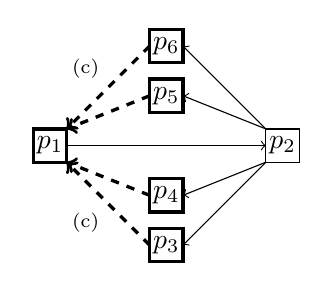
\begin{tikzpicture}[scale=1.2]

  \newcommand\X{35pt};
  \newcommand\Y{15pt};

  \scriptsize
  \draw[->](5+0*\X, 0*\Y) -- (-5+ 2*\X, 0*\Y);
  \draw[->] (-5+2*\X, 5pt) -- (5+\X, \Y);
  \draw[->] (-5+2*\X, 5pt) -- (5+\X, 2*\Y);
  \draw[->] (-5+2*\X, -5pt) -- (5+\X, -\Y);
  \draw[->] (-5+2*\X, -5pt) -- (5+\X, -2*\Y);

  \draw[->,dashed, very thick](-5+\X, 2*\Y) --
  node[anchor=south east]{(c)} ( 5pt,5pt);
  \draw[->,dashed, very thick](-5+\X, 1*\Y) -- ( 5pt,5pt);
  \draw[->,dashed, very thick](-5+\X, -1*\Y) -- ( 5pt,-5pt);
  \draw[->,dashed, very thick](-5+\X, -2*\Y) --
  node[anchor=north east]{(c)}( 5pt,-5pt);

  \normalsize
  \draw[fill=white, very thick]
  (0*\X, 0*\Y) node{$p_1$} +(-5pt,-5pt) rectangle +(5pt,5pt);
  \draw[fill=white]
  (2*\X, 0*\Y) node{$p_2$} +(-5pt,-5pt) rectangle +(5pt,5pt);

  \draw[fill=white, very thick]
  (1*\X,2*\Y) node{$p_6$} +(-5pt,-5pt) rectangle +(5pt,5pt);
  \draw[fill=white, very thick]
  (1*\X,1*\Y) node{$p_5$} +(-5pt,-5pt) rectangle +(5pt,5pt);
  \draw[fill=white, very thick]
  (1*\X,-1*\Y) node{$p_4$} +(-5pt,-5pt) rectangle +(5pt,5pt);
  \draw[fill=white, very thick]
  (1*\X,-2*\Y) node{$p_3$} +(-5pt,-5pt) rectangle +(5pt,5pt);
 

\end{tikzpicture}}
  \caption{\label{fig:joiningexample}Example of the \SPRAY's joining
    protocol.}
\end{figure*}


The sole representative of adaptive-by-design random peer sampling is
\SCAMP~\cite{ganesh2001scamp,ganesh2003peer} which stands for
SCalable Membership Protocol. Its interesting property lies in its
logarithmically growing partial view sizes meeting the sharp threshold
of connectedness of random
graphs~\cite{erdos1959random}. Nevertheless, \SCAMP suffers from
other flaws. In particular, it systematically performs random walks to
establish its connections. In the WebRTC context, each random walk
must be traveled back to finalize the connection establishment as
illustrated in figure~\ref{fig:webrtc}. It drastically impacts on the
\SCAMP failure probability of establishing a connection. Indeed, let
$P_f$ the probability of either the peer or the link between the
latter and the next peer crashes/disconnects when it holds the
traveling message, without any possible recovery. Let $P_E$ the
probability that a connection establishment cannot be
completed. Without three-way handshake, $P_E$ is straightforward:
\begin{equation} P_{E,\,1way}^{Scamp}=1-(1- P_f)^{k+1} \end{equation} where $k$
is the number of hops before the end of the random walk with a minimum of $2$
hops. On the other hand, in the handshaking context, the message must travel
back to its origin in order to be completed. As consequence, when a
subscription travels through a peer or a link, they are not allowed to fail
until the subscription travels back. Thus, we obtain:
\begin{align} P_{E,\,3way}^{Scamp} &=1 - ((1-P_f)^{2(k+1)} (1-P_f)^{2k}
                                     \ldots (1-P_f)^2) \nonumber \\
                                   &=1-(1-P_f)^{k^2+3k+2}
\end{align}
The complexity class of the \SCAMP failure rate increases leading to a quick
degenerating number of connections over time. This behavior endangers the
network connectedness.

Building an adaptive-by-design random peer sampling that meet WebRTC
constraints raises the following scientific problem:

\begin{problem}
  Let $t$ be an arbitrary time frame, let $\mathcal{N}^t$ be the
  network membership at that given time $t$ and let $\mathcal{P}_x^t$
  be the partial view of peer $p_x \in \mathcal{N}^t$.  A
  cost-efficient random peer sampling should provide the following
  best-case properties:
  \begin{enumerate}
  \item  \begin{center}
    Partial view size: \hfill
    $\forall p_x \in \mathcal{N}^t,\, |\mathcal{P}_x^t| = \Theta (\ln
    |\mathcal{N}^t|)$
  \end{center}
  
\item \begin{center}
    Connection establishment: \hfill $O(1)$
  \end{center}
 
\item  \begin{center}
    Convergence speed: \hfill $\Theta(\exp \, t^{-1})$
  \end{center}
  \end{enumerate}
\end{problem}

The first condition states that partial view size is relative to size of the
network at any time. It also states that partial views grow and shrink
logarithmically compared to the size of the network. The second condition
states that each connection establishment requires a constant number of
intermediary peers. Since this number is constant, connections establishments
do not depend of the network size. The last condition states that the network
overlay converges exponentially fast to a topology exposing properties similar
to random graphs.  \CYCLON and \SCAMP fail to fulfill the first condition
and the second condition, respectively.

%%% Local Variables:
%%% mode: latex
%%% TeX-master: "../paper"
%%% End:
